\chapter{Besoins de l'utilisateur}
{
\begin{figure}[H]
    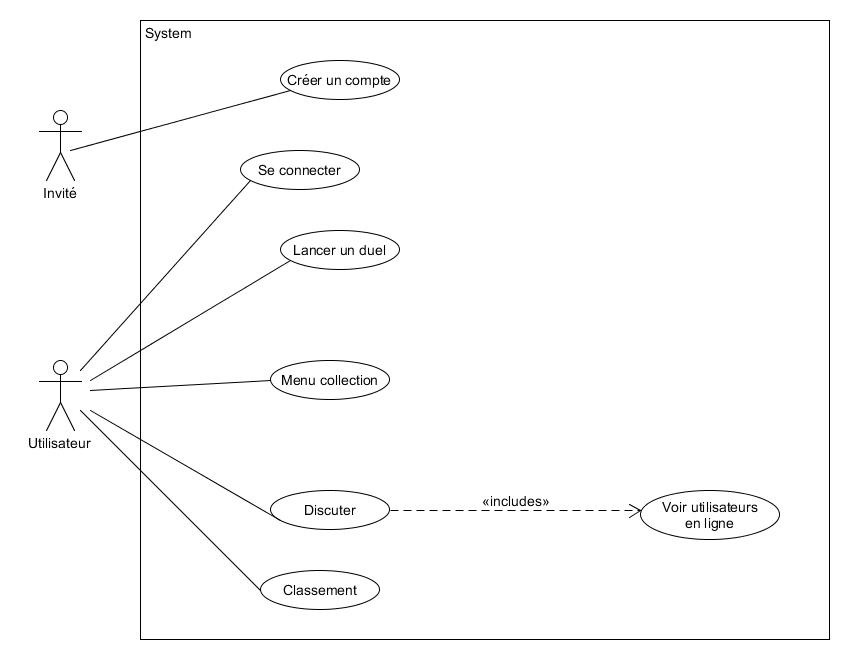
\includegraphics[width=1\textwidth,height=1\textwidth]{Images/useCase.jpg}
    \caption{\label{Use case view}Use case view}
\end{figure}
}

\section{Exigences fonctionnelles}
\iffalse
\subsection{Gestion des clients}
\begin{itemize}
    \item Cas général  : Le client doit pouvoir s'inscrire ou se connecter sur le \index{serveur}serveur avec un nom d'utilisateur unique et un mot de passe associé à celui-ci.
    \item Conditions  : Voir \hyperref[insc]{Inscription} ou \hyperref[connec]{Connexion} pour les conditions specifiques.
    \item Cas Exceptionnel : Lors d'un erreur celui ci sera traite par son cas d'utilisation unique telle que \index{inscription}Inscription ou \index{connexion}Connexion.
\end{itemize}
\fi
\subsection{Inscription\index{inscription}}\label{insc}
\begin{itemize}
    \item Cas général  : Création d'un nouveau compte\index{compte} via un nom d'utilisateur\index{utilisateur} unique et un mot de passe.
    \item Pré condition  : L'utilisateur ne possède pas de compte.
    \item Post condition : Un nouveau compte est créé sur le serveur\index{serveur}.
    \item Cas exceptionnel : Nom d'utilisateur déjà utilisé, l'utilisateur est averti et redirigé.
\end{itemize}
\subsection{Connexion\index{connexion}}\label{connec}
\begin{itemize}
    \item Cas général : Connection au serveur avec un identifiant et un mot de passe.
    \item Pré condition  : L'utilisateur\index{utilisateur} n'est pas connecté.
    \item Post condition : L'utilisateur est connecté au serveur.
    \item Cas exceptionnel : Les données introduites sont incorrectes, le serveur\index{serveur} averti le client\index{client} et celui-ci est amené à reessayer.
\end{itemize}
\subsection{Classement\index{classement}}
\begin{itemize}
    \item Cas général : L'utilisateur\index{utilisateur} consulte le classement des différents joueurs.
    \item Pré condition : L'utilisateur est connecté et est dans le menu adéquat.
    \item Post condition : L'utilisateur a consulté le classement.
\end{itemize}
\subsection{Créer un deck\index{deck}}
\begin{itemize}
    \item Cas général : Création d'un nouveau deck avec les cartes de sa collection\index{collection}.
    \item Pré condition  : L'utilisateur est connecté au serveur et il ne possède pas 5 decks complets.
    \item Post condition : Le deck contient 20 cartes et respecte les conditions d'un deck.
\end{itemize}
\subsection{Matchmaking\index{matchmaking}}
\begin{itemize}
    \item Cas général : L'utilisateur\index{utilisateur} lance la recherche d'adversaire\index{adversaire}.
    \item Pré condition  : L'utilisateur est bien connecté au serveur.
    \item Post condition : Un adversaire a été trouvé, et la liaison est créée.
\end{itemize}
\subsection{Jouer un tour}
\begin{itemize}
    \item Cas général : L'utilisateur\index{utilisateur} effectue éventuellement des actions et termine son tour.
    \item Pré condition  : Le joueur est en train de disputer un duel\index{duel}.
    \item Post condition : Ce n'est plus son tour de jouer.
    \item Cas exceptionnel :  Déconnection brutale d'un des joueurs. Forfait\index{forfait} pour le joueur déconnecté.
\end{itemize}
\subsection{Abandonner}
\begin{itemize}
    \item Cas général : L'utilisateur\index{utilisateur} peut déclarer forfait durant un duel.
    \item Pré condition  : C'est le tour de l'utilisateur.
    \item Post condition : Défaite et mise à jour du classement\index{classement}.
\end{itemize}

